\documentclass[11pt]{article}
\usepackage[margin=1in]{geometry}
\usepackage[T1]{fontenc}
\usepackage{lmodern,amsmath,amssymb,amsthm,booktabs,array,graphicx,xcolor}
\usepackage{xurl}
\usepackage[colorlinks=true,linkcolor=blue!45!black,citecolor=blue!45!black,urlcolor=blue!45!black]{hyperref}
\usepackage{microtype}
\newtheorem{theorem}{Theorem}
\newtheorem{proposition}[theorem]{Proposition}
\newcommand{\F}{\mathbb F}
\newcommand{\ev}[1]{\textup{[#1]}}
\newcommand{\AS}{\operatorname{AS}}
\title{Exact Norm-Based Search for Constrained Roots over Finite Fields:\\
Predicates, Circuit Representations, and Bounded Evidence}
\author{Anonymous}
\date{Research draft --- October 17, 2026}
\begin{document}
\maketitle
\begin{abstract}
We study a search architecture for constrained finite-field roots that separates
exact algebraic predicates, representation cost, and complete solution enumeration.
For a binary elliptic-curve norm chart with five source coordinates, we give an
explicit parametrization using the sources, one field parameter, and one
Artin--Schreier kernel bit. We prove its coefficient-identity contract, including
zero and repeated sources. A bounded affine-cone compiler preserves primary
assignments by a unique functional extension, while exposing the cost of a native
solver's internal XOR decomposition. On one fixed $\F_{2^{83}}$ instance, a
representation change reduces post-flush native coordinates from 58,176 to
45,427. A subsequent bounded search returns UNKNOWN with no verified witness.
A characteristic-independent nilpotence criterion and existing supplied-polynomial
tests explain which components extend to odd fields. These results establish
exact component contracts and a representation improvement; they do not establish
a complete replacement for Gr\"obner-basis solving, a speedup over F4/F5/F6, or a
new asymptotic bound. We give the missing completeness bridges, an explicit
performance gate, and a reproducible next experimental queue.
\end{abstract}
\section{Problem, scope, and contribution}
Let $K$ be a finite field, $D_i\subseteq K$ finite constrained domains, and
$f_1,\ldots,f_s\in K[X_1,\ldots,X_m]$. The generalized root-finding task is to
return the entire ordered set
\[
 {\cal Z}=\{(x_1,\ldots,x_m)\in D_1\times\cdots\times D_m:
                    f_j(x_1,\ldots,x_m)=0\text{ for every }j\}.
\]
An exact all-roots implementation must establish both membership and coverage.
If auxiliary variables occur in the input system, the requested projection and
whether auxiliary fibers must be returned are part of the input contract.
Finding a witness, completing a relaxation, and enumerating a projected norm
chart are different tasks.

The motivating application is the constrained polynomial-system stage of
elliptic-curve index calculus. Semaev's summation polynomials provide an algebraic
connection to point relations \cite{semaev}. The implementation considered here
instead searches a structured norm identity before reconstructing original
chain solutions. This manuscript documents that narrower implemented stage.
It is distinct from the repository's earlier \texttt{rootfinding-decomposition}
manuscript about direct subtraction and pair tables at smaller decomposition
orders. Its measurements and reported ratios are not imported here.

There are three concrete contributions. First, Theorem~\ref{thm:chart} gives
an exact binary norm-chart contract and a short coefficient proof that avoids
generic-position divisions. Second, Theorem~\ref{thm:compiler} explains why
bounded affine substitution changes representation without changing primary
models. Third, the measured native-coordinate profile and the subsequent
negative search result demonstrate that fewer declared variables need not
produce a hard-instance solution. These are mathematical exposition and
engineering results assembled from versioned artifacts, with no priority claim
for the underlying algebra or SAT techniques.

\subsection{Related work and the novelty boundary}
F4 organizes Gr\"obner-basis reductions using linear algebra
\cite{f4}; F5 introduces signature-based avoidance of reductions to zero
\cite{f5}. A comparison must identify an actual implementation, field backend,
input ideal, and final all-roots output, rather than compare algorithm labels.
The program also requires the repository-specific F6 baseline. This draft
does not identify a canonical F6 publication or establish that its available
interface matches the full root contract.

SAT with XOR reasoning and coordinated changes to representation are established
techniques \cite{cms}. Particularly close prior work is
Trimoska--Ionica--Dequen's WDSat approach to index-calculus systems
\cite{wdsat}, including ANF-aware parity reasoning and branching intended to
expose linear structure. Consequently, neither using SAT instead of Gr\"obner
bases nor branching on primary variables is a novelty claim here.
A full comparison of their mathematical model, preprocessing, and branching
against this norm parametrization remains necessary before submission.

Finite-field factorization and Frobenius computation are classical
\cite{cz,frobenius}. The support criterion below is an elementary consequence
of multiplicities in a quotient ring. Factoring an already supplied quintic
does not solve the search over its unknown coefficients. Our candidate research
advance would have to be a demonstrably useful structural reduction or pruning
rule beyond these ingredients. That advance, and its qualified end-to-end
performance, remain open.

\section{Exact algebraic contracts}
\subsection{Repeated-root-safe domain support}
Let $D\subseteq K$ be finite and let
$L_D(X)=\prod_{d\in D}(X-d)$. The empty product is one.

\begin{theorem}[Support by nilpotence]\label{thm:support}
For a monic $H\in K[X]$ of degree $m\geq1$ and an integer $k\geq m$,
every root of $H$ in an algebraic closure lies in $D$ if and only if
\[
          (L_D\bmod H)^k=0\quad\text{in }K[X]/(H).
\]
\end{theorem}
\begin{proof}
Write $H=\prod_\alpha(X-\alpha)^{e_\alpha}$ over an algebraic closure.
The displayed equality is equivalent to $H\mid L_D^k$. The roots of $L_D$
are precisely the elements of $D$, each with multiplicity one. Divisibility
therefore holds exactly when every $\alpha\in D$ and every $e_\alpha\leq k$.
The second condition follows from $e_\alpha\leq m\leq k$.
Divisibility over the algebraic closure is equivalent to divisibility over
$K$ by the remainder theorem for monic division.
\end{proof}

The nonconstant hypothesis matters: a constant monic $H=1$ has no roots and
must be handled as a separate trivial case. If $D$ is empty, the criterion
rejects every nonconstant $H$. Squarefreeness of $H$ is not assumed.
In characteristic $p$ one may take $k=p^{\lceil\log_p m\rceil}$.
For a binary quintic, $k=8$ suffices, as in the compact support oracle \ev{E1}.
This supplies an exact predicate, not a bound on how many coefficient
candidates must be searched.

For a binary linear space $V$ and $v\notin V$,
\[
 L_{V+\F_2v}(X)=L_V(X)L_V(X+v)
              =L_V(X)^2+L_V(v)L_V(X).
\]
Indeed the two cosets are disjoint, and induction starting at $L_{\{0\}}=X$
shows that $L_V$ is additive. For an affine space $a+V$, substitute $X-a$.
These formulas can represent an exponentially large binary domain implicitly.
They do not give a proper nonzero $\F_p$-linear subspace of the prime field
$\F_p$; an interval or another domain representation is required there.

In an extension field, Frobenius acts on coefficients too:
$(\sum c_iX^i)^p=\sum c_i^pX^{ip}$. It is $\F_p$-linear, generally not
$K$-linear. For example, in $\F_4$ with $\omega^2=\omega+1$,
the square of the constant $\omega$ is $\omega+1$, not $\omega$.
In odd characteristic an ordinary square also contains cross terms.
Neither binary shortcut can be transplanted unchanged to an odd-field backend.

\subsection{A binary elliptic-curve norm chart}
Throughout this subsection $K=\F_{2^n}$ and
\[
 E:\quad Y^2+XY=C(X),\qquad C(X)=X^3+aX^2+b,\qquad b\ne0.
\]
Fix $T=(z,y_T)\in E(K)$ with $z\ne0$. For $r,s,h,k\in K$ set
\begin{equation}
 \begin{split}
 P&=X^3+rX^2+sX+t,\qquad Q=hX+k,\\
 t&=z^3+rz^2+sz+(hz+k)y_T,\\
 N&=P^2+XPQ+Q^2C .
 \end{split}
\end{equation}
Conjugation in the quadratic function-field equation sends $Y$ to $Y+X$,
so $N$ is the norm of $P+QY$. The chosen $t$ makes $(P+QY)(T)=0$;
hence $N(z)=0$. Its leading coefficient is one and its degree is six.
Thus $H=N/(X+z)$ is a monic quintic.

Given ordered source values $x_1,\ldots,x_5\in K$, write
\[
 H_x=\prod_{i=1}^5(X+x_i)
     =X^5+e_1X^4+e_2X^3+e_3X^2+e_4X+e_5.
\]
Let $\beta=\sqrt b$, $c=(y_T+\beta)/z$, and $w=\sqrt{e_5/z}$.
Square roots are unique because Frobenius is an automorphism of $K$.

\begin{theorem}[Exact norm-chart parametrization]\label{thm:chart}
The identity $N=(X+z)H_x$ is equivalent to the following conditions:
\begin{align}
 h^2+h&=e_1+z,                                             \label{eq:as}\\
 k&=e_2+r^2+hr+ah^2+ze_1,                                 \label{eq:k}\\
 s&=zr+ck+y_Th+z^2+w,                                     \label{eq:s}\\
 0&=R_3:=e_3+hs+kr+k^2+ze_2,                              \label{eq:r3}\\
 0&=R_4:=\beta k^2+(zw)k+e_5+ze_4.                        \label{eq:r4}
\end{align}
No hypothesis excludes $h=0$, $k=0$, zero sources, or repeated sources.
\end{theorem}
\begin{proof}
The coefficients of $N$, in descending order, are
\[
\begin{array}{c|l}
6&1\\
5&h+h^2\\
4&r^2+k+hr+ah^2\\
3&kr+hs+k^2\\
2&s^2+ks+ht+bh^2+ak^2\\
1&kt\\
0&t^2+bk^2 .
\end{array}
\]
Comparison at degrees five, four, and three gives
\eqref{eq:as}, \eqref{eq:k}, and \eqref{eq:r3}.
The constant coefficient identity is $t^2+bk^2=ze_5$, or
$t=\beta k+zw$; substituting the definition of $t$ and dividing by the
nonzero $z$ gives \eqref{eq:s}. The coefficient at degree one becomes
\eqref{eq:r4}. This proves necessity.

Conversely these equations match every coefficient except possibly degree two.
The difference $N+(X+z)H_x$ is therefore $AX^2$ for some $A\in K$.
Both polynomials vanish at $z$, giving $Az^2=0$. Since $z\ne0$, $A=0$.
This proves sufficiency without another division or a generic-position
assumption.
\end{proof}

The map $\AS(h)=h^2+h$ is $\F_2$-linear with kernel $\{0,1\}$ and
image dimension $n-1$. Choose any fixed linear section $S$ on this image.
For arbitrary inputs $e_1$, extend the section linearly to $K$ and check
the explicit residual \eqref{eq:as}. Then
\[
                  h=S(e_1+z)+\eta,\qquad \eta\in\F_2
\]
enumerates each valid $h$ exactly once. This works for even as well as odd
$n$; an odd-degree half-trace formula is not an all-extension implementation.
Once the sources, $r$, and $\eta$ are fixed, \eqref{eq:k} and
\eqref{eq:s} determine $k,s$ uniquely. The explicit residuals then accept
exactly the norm identities. For a $d$-dimensional binary source space,
the primary description has $5d+n+1$ bits \ev{E1--E3}; the actual
$n=83,d=18$ fixture uses 174.

This bijection concerns norm witnesses with the specified target and degree
chart. The target branch $z=0$ is outside the theorem. A norm factor can
correspond to the conjugate point above a source coordinate, and special
divisors and chain auxiliary fibers require separate analysis. The theorem
does not imply that these 174-bit models are in bijection with the original
339-variable chain solutions.

\section{Search, representation, and output semantics}
\subsection{Norm-primary enumeration}
The implemented search \ev{E3} compiles the three zero residuals
\eqref{eq:as}, \eqref{eq:r3}, and \eqref{eq:r4}, together with the functional
field operations, into a Boolean arithmetic DAG. Field parameters and the
domain basis are fixed inputs. A primary-only decision policy is enforced
in a source-pinned native CryptoMiniSat fork; auxiliary coordinates still
participate in propagation and Gaussian elimination.

\begin{center}
\fbox{\begin{minipage}{0.92\linewidth}
\textbf{Algorithm 1: exact norm-primary enumeration with a budget.}\\
1. Validate the field, curve, target, and domain; require $z\ne0$.
Build the elementary coefficients and the functional parametrization.\\
2. Compile the residuals with the declared affine-support limit.
Initialize the native solver with the primary decision mask.\\
3. On SAT, replay every declared coordinate against its unique functional
extension; check every CNF/XOR relation and the original arithmetic DAG.
Independently form the literal polynomial norm and divide by $X+z$.\\
4. Retain the verified norm witness. Block the entire primary assignment
and repeat. A duplicate or failed replay is an error.\\
5. On native UNSAT, report complete enumeration of this norm-primary
predicate, conditional on solver correctness. On UNKNOWN, a model cap,
or an expired budget, return verified witnesses as a lower bound with the
exact count unset. Keep original-system completeness unset.
\end{minipage}}
\end{center}

Soundness follows from Theorem~\ref{thm:chart} and independent replay.
The full-primary blocking clause removes exactly the emitted assignment.
Induction gives distinct witnesses and no removal of an unreported primary
assignment. Exhaustion of the remaining predicate therefore establishes
coverage within the norm chart, conditional on the solver's UNSAT verdict.
The implementation does not supply an independently checked large UNSAT
certificate; native exhaustion is not advertised as certified generalized
root finding.

There are at most $2^{5d+n+1}$ primary assignments. Exhaustive functional
evaluation is a finite reference method, but this bound is exponential.
The SAT implementation has no established polynomial or subexponential
worst-case advantage. Storage includes the compiled DAG, solver state,
and emitted witnesses; learned-clause growth is not bounded here by a small
polynomial guarantee. Output enumeration itself can require exponential time.

\begin{figure}[tb]
\centering
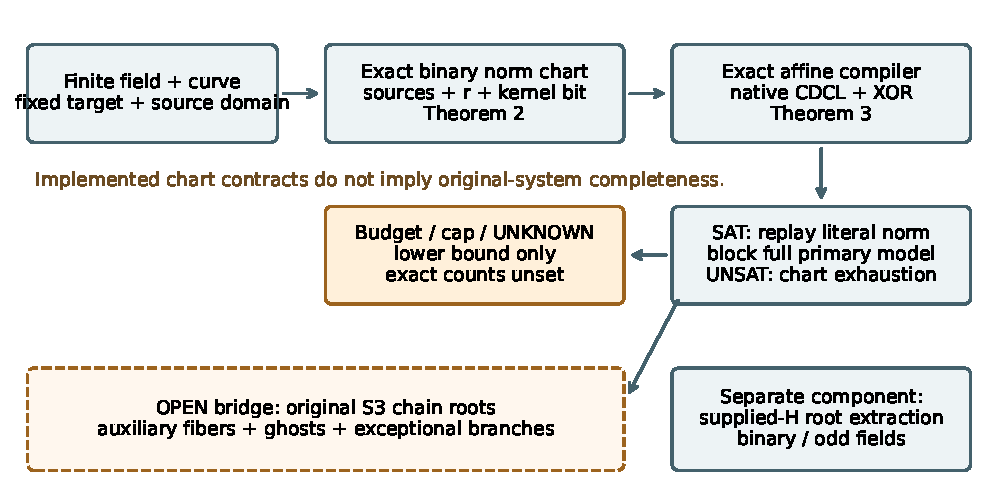
\includegraphics[width=\linewidth]{figures/architecture.pdf}
\caption{Contract boundaries. Exact chart enumeration and supplied-polynomial
root extraction are implemented components. The original-system reconstruction
bridge and an independently certified complete hard search remain open.
An interrupted search returns a lower bound, not an exact count.}
\label{fig:architecture}
\end{figure}

\subsection{Bounded affine cones}
At a binary XOR wire, represent the value as an affine form over already
defined primary atoms, nonlinear outputs, and retained linear atoms.
Addition is symmetric difference of supports, with a separately retained
constant bit. When the declared support limit is exceeded, introduce a
shared parity alias with its exact XOR definition. At an AND retain the
exact three-clause gate definition on signed input aliases and a fresh output.
Constant wires and empty parity contradictions must remain exact.

\begin{theorem}[Unique extension under affine contraction]\label{thm:compiler}
For an acyclic functional Boolean DAG and the transformation just described,
every primary assignment has exactly one extension satisfying the introduced
definitions. That extension has the same final residuals as the original DAG.
Projection of satisfying assignments to primary coordinates is a bijection
between the transformed and original predicates.
\end{theorem}
\begin{proof}
Order the construction topologically. Every new coordinate is defined as a
specified parity or AND of earlier coordinates, so its value exists and is
unique after those coordinates are fixed. Induction proves that every affine
form denotes its original wire value, including the constant phase and
cancellation to an empty support. The same induction applies conversely to
any satisfying assignment of the defining constraints: its new coordinates
must equal those values. Final zero constraints therefore agree exactly,
which proves both directions and uniqueness.
\end{proof}

The support limit controls the representation, not a relaxation of
nonlinear multiplication. Dense affine forms can shrink the number of
external variables while dramatically expanding native internal XOR cuts.
For the pinned two-input cut construction the profile estimates additional
coordinates per row by
$\lfloor\max(\ell-3,0)/2\rfloor$, where $\ell$ is row length \ev{E2}.
This is a source-specific pre-cleaning estimate, not a portable SAT theorem.
Actual post-flush counts are recorded separately. The compiler proof gives
no monotonic relation between either count and solution time.

\subsection{Permutation representatives}
\begin{proposition}[Source symmetry]\label{prop:symmetry}
If all five source domains equal $D$, and the tested predicate depends on
the sources only through $H_x$, sorting the five encoded source coordinates
selects one representative of each source-permutation orbit. Restoring
every distinct permutation, with the remaining primary parameters fixed,
recovers the full ordered norm-primary set.
\end{proposition}
\begin{proof}
The product $H_x$ is invariant under permutations. A fixed total order on
the finite coordinate encoding gives exactly one nondecreasing tuple for
each multiset. Every ordered tuple with this multiset is a distinct
permutation of that representative. These sets are disjoint for different
multisets. Parameters $r,\eta$ are unaffected by permutation, so the same
argument holds independently at each parameter pair.
\end{proof}

An orbit with source multiplicities $m_j$ has size $5!/\prod_jm_j!$.
Repeated sources preclude division of a model count by a uniform 120.
This proposition does not apply to arbitrary nonsymmetric $f_j$, unequal
domains, or chain auxiliaries without another invariance proof.
The orbit restoration oracle is implemented and tested \ev{E4}.
A sorted-source comparator in the actual hard native search is a next
experiment, not a result of the current worker.

\section{Recorded evidence}
All values in this section are transcribed from frozen native artifacts,
identified in Appendix~\ref{app:artifacts}. This paper build introduces no
new solver experiment or timing measurement. Counts of assignments below
are component correctness controls, not independent hard benchmark instances.

\subsection{Independent small oracles and field coverage}
The original norm compiler records 73,216 complete primary assignments
across eight small $\F_4,\F_8,\F_{16}$ models \ev{E1,E2}.
The bounded-cone transformation records 116,480 complete-assignment checks
in $\F_4,\F_8$ across its seven limits. Seven native complete enumerations
agree on a 28-model fixture \ev{E2}. The changed search driver records
2,048 independent literal-norm assignments and six complete 28-model native
sets, plus cap-one and expired-budget checks \ev{E3}.
These panels vary target signs and include even extensions and zero or
repeated sources. Literal polynomial arithmetic is independent of the
compiler equations; it is not an independent author's replay.

The symmetry preparation records 34,816 literal assignments over eight
small cases \ev{E4}. Six cases restore 28 ordered norm-primary witnesses
from six sorted representatives; two restore 168 from fifteen. Orbit
sizes include one, five, ten, and thirty. All restored sets agree exactly
with the full literal sets. No timing ratio is inferred from these counts.

\begin{table}[tb]
\centering\small
\begin{tabular}{p{0.23\linewidth}p{0.34\linewidth}p{0.33\linewidth}}
\toprule
Component & Recorded field coverage & Established scope\\
\midrule
Binary norm chart and compiler & Tiny binary extensions; one actual
$\F_{2^{83}}$ search fixture & Primary-predicate equivalence and bounded
search diagnostics \ev{E1--E3}\\
Source symmetry & $\F_4,\F_8$, eight cases & Exact norm orbit restoration;
no hard comparator search \ev{E4}\\
Odd supplied-quintic adapter & Eleven odd fields, including all five
NIST prime sizes & Roots and multiplicities of supplied polynomials;
no multivariate coefficient search \ev{E5}\\
\bottomrule
\end{tabular}
\caption{Field coverage is stated per component. It does not certify a
comprehensive all-roots solver across these fields.}
\label{tab:coverage}
\end{table}

The odd adapter first forms $G=\gcd(H,X^q-X)$, where $q=|K|$,
then splits this squarefree product of all distinct field-root factors.
It verifies that the product of returned distinct linear factors is exactly
$G$; exact division in $H$ recovers multiplicities. A bounded splitting
failure returns unresolved. This is classical finite-field factoring,
with a coverage certificate for a supplied polynomial, rather than a new
multivariate algorithm.

The recorded wide test comprises 66 known-answer quintics over eleven
fields: $\F_3$, $\F_5$, $\F_7$, $\F_{11}$, $\F_9$, $\F_{25}$, and the prime fields
of NIST P-192, P-224, P-256, P-384, and P-521 \ev{E5}.
The five prime interval widths are respectively 40, 47, 53, 79, and 106
bits. The adapter also records 3,624 tiny-field controls with independent
Hasse-derivative multiplicities. These tests cover repeated and nonrational
factors. They demonstrate a supplied-polynomial component at large
characteristics; they do not establish a corresponding prime-field norm
search, all scale sizes, or every index-calculus implementation.

\subsection{Actual binary instance and representation profile}
The fixed fixture \ev{E0} uses
\[
 \begin{split}
 K&=\F_2[\theta]/(\theta^{83}+\theta^{45}+\theta^2+\theta+1),\\
 D&=\operatorname{span}_{\F_2}\{1,\theta,\ldots,\theta^{17}\},\\
 E&:\quad Y^2+XY=X^3+1 .
 \end{split}
\]
The full curve identifier is
\texttt{icv1-f2m83-tm6151469093347-debefd74}.
It is a recorded binary fixture, not a named NIST binary-curve preset.
Its original five-source chain contains 339 Boolean variables and 332
equations; the norm chart has 174 primary bits. These dimensions do not
prove equivalence of the two complete solution sets.

\begin{table}[tb]
\centering\small
\begin{tabular}{lrrrr}
\toprule
Support limit & External & XOR rows & Actual internal & Pre-clean estimate\\
\midrule
1 &58,176&44,921&58,176&58,176\\
2 &40,148&26,893&45,427&45,427\\
4 &30,509&17,254&55,395&55,395\\
8 &26,389&13,134&74,121&74,121\\
16&23,754&10,499&106,094&106,094\\
32&22,121&8,866&not loaded&161,033\\
Dense&16,134&2,879&not loaded&910,133\\
\bottomrule
\end{tabular}
\caption{Native cut-aware representation profile \ev{E2}. All arms have
174 primary variables and 39,742 CNF clauses before native XOR cuts.
The last two exceed the preregistered 150,000-coordinate estimate cap.
There is no SAT solve or Gaussian initialization in this profile.}
\label{tab:profile}
\end{table}

\begin{figure}[tb]
\centering
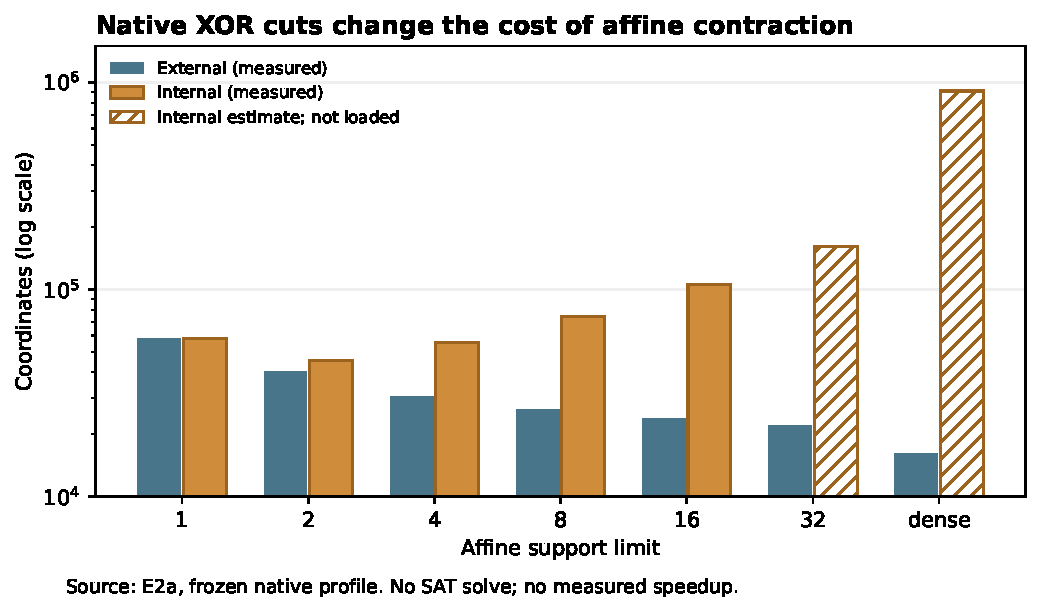
\includegraphics[width=\linewidth]{figures/native_coordinates.pdf}
\caption{Recorded variables for the fixture identified above \ev{E2}.
Measured post-flush internal counts are shown only for loaded arms.
Hatched bars are estimates for capped arms, not measurements. Logarithmic
scale exposes native expansion. Coordinate reductions are not speedups.}
\label{fig:profile}
\end{figure}

Limit two has 21.9\% fewer actual native coordinates than limit one
(Table~\ref{tab:profile}). Dense substitution has the smallest external
count and the largest pre-cleaning internal estimate. This refutes use of
the external variable count alone as the representation-selection criterion.
Limit two was selected after observing this training profile; it is not
a holdout winner.

\subsection{Hard search: a negative bounded result}
The next preregistered worker \ev{E3} asked whether the changed limit-two
representation would produce at least one replayed norm witness or complete
norm exhaustion within its 60-second inner budget. It did neither.
The supervisor records 61.794 seconds cold wall lifetime and 385,368 KiB peak
process RSS. The native inner lifetime is 61.510 seconds, including its
reported overshoot. These are development diagnostics; qualified exclusive
isolation and a matched baseline were not established.

The final verdict is UNKNOWN, with zero verified norm witnesses, null exact
norm count, and null original-system count. One Gaussian matrix was
initialized, peaking at 9,169 rows and 22,491 columns; no row or column
admission cap was rejected. The record includes 7,167 conflicts,
12,065 primary decisions, zero auxiliary decisions, and 28,207,875 Gaussian
row XORs \ev{E3}. The evidence narrows the failure: matrix admission occurred,
but useful search completion did not follow within the budget. It does not
show that a witness is absent.

The worker used one CPU, a 4 GiB per-process address-space cap, a 90-second
outer supervisor, and a 4,096-model output cap. Successful process exit only
means that the diagnostic envelope was serialized. The bounded first-witness
prediction is refuted; the general research objective is still open.
No ratio against an earlier timeout or a Gr\"obner baseline is computed.

\section{Limitations, corrections, and the next falsifiable step}
\subsection{Completeness and certification obligations}
A generalized replacement must cover the input system, not just this norm
chart. The remaining bridge includes original summation-chain auxiliary
fibers, exceptional maps, $z=0$, rational lifts versus conjugate or
ghost norm configurations, and all branch multiplicities. Each branch
needs an exact original-system validator and a coverage argument. Testing
a supplied $H$ or rejecting sampled relaxed norms cannot close the
coefficient-search problem: the recorded divisor relaxation still has
$2^{73}$ candidates at fixed parameters \ev{E1}.

Theorem~\ref{thm:support} is valid over every finite field.
Theorem~\ref{thm:chart} is explicitly characteristic two. Koblitz curves are
a structured binary subclass, not a third field characteristic. Applicable
binary formulas still require a field representation, valid curve parameters,
and the theorem's target hypotheses. Prime curves require an odd-characteristic
chart and an appropriate domain representation. Large-prime supplied-quintic
validation is useful infrastructure, but does not fill that gap.
No statement here establishes an efficient universal algorithm at arbitrary
sizes.

All theorems have readable proofs in this manuscript, but no checked Lean
formalization is supplied. The local commands \texttt{lean} and
\texttt{conductor} are unavailable in the manuscript environment; that is a
specific tooling limitation, not a proof or a reservation. The central
formalization obligation is the coefficient identity together with its
finite-field square-root and Artin--Schreier hypotheses. The separate existing
Lean proof in the earlier decomposition manuscript is not a proof of these
theorems. Appendix~\ref{app:artifacts} maps the outstanding obligations.

The repository's current \texttt{identity.certificate/v1} checker evaluates
unconditional identities modulo $2^{61}-1$. It cannot faithfully certify the
characteristic-two identities or conditional implications here by merely
changing a label. We therefore attach source-hashed native evidence pointers
and the written proofs, with this certificate-format gap stated explicitly.
No such certificate or formal verification is claimed.

\subsection{Preserved erratum}
A prior transfer-only proof omitted a term. The correction \ev{E6} is
\[
 \begin{split}
 V=e_5+e_1e_4
   &=(h^2+h)e_4\\
   &\quad+k(zs+z^2r+ky_T+z^3+hz y_T).
 \end{split}
\]
Thus $k=0$ does not generally imply $V=0$.
Over $\F_4$ with $\omega^2=\omega+1$, take $a=0,b=1$, target
$(z,y_T)=(1,0)$, and $h=\omega,k=r=s=0$. Literal division gives
$H=X^5+X+1$, so $e_1=0$ and $e_4=e_5=1$, hence $V=1$.
This counterexample invalidates the omitted-term formula.
Generic support code computes the coefficients directly and does not use
that simplification. Historical files remain preserved; the correction
must travel with any use of the old transfer argument.

\subsection{Performance gate and comparison still owed}
The program requires twenty preregistered hard matching instances, completed
all-roots outputs on every method, a fastest baseline taking at least one
second, and at least three cold repetitions. Genuine source-identified
F4/F5/F6 interfaces must return the same original roots. The immutable floor
is at least a twofold geometric-mean end-to-end gain, no more than 1.10 worst
slowdown, A/A variation at most 10\%, qualified isolation, and the requested
field coverage \ev{E7}. The higher requested speed targets are research
objectives, not achieved results. Nothing in this manuscript passes the floor.

Comparisons still owed include strong available systems such as Magma,
msolve, FGb, Singular, and OpenF4, subject to field and contract support.
The supplied-polynomial stage also owes a matched comparison against
established factorization implementations such as FLINT, NTL, or Magma.
Baseline tuning, conversion, setup, solving, extraction, verification, and
serialization must all be charged consistently. Unsupported fields are
reported, not silently replaced with easier ideals. Native SAT is not
itself an F4/F5/F6 baseline.

\subsection{Next queue}
The failed prediction leads to a changed experiment, not an identical rerun.
The first queued variant is sorted-source norm-primary search:
add an exact comparator network for the canonical source encoding, prove its
unique extensions, enumerate representatives, and restore every distinct
permutation. Before a hard run, require exact agreement with all eight
symmetry-oracle sets \ev{E4}, including zero and repeated sources.
Freeze the comparator source, input digest, native source manifest, budgets,
and decision mask. Predict a verified witness or representative exhaustion
on the same actual fixture within a bounded inner search; on failure,
retain UNKNOWN and move to a structural variant. At most three experiments
may be scheduled in a bounded session, each at one core and 4 GiB.

The second route is conditional whole-cell pruning using the support
nilpotence equations, rather than enumerating all relaxed divisors.
A proposed cell certificate must imply rejection of every point in that
cell; rejection of random sample norms is insufficient. Its small oracle
must compare complete cell membership and cover repeated factors.
The third route develops an odd-characteristic norm parametrization with
a separate prime-domain contract. It must preserve odd cross terms and
prove exceptional branches before importing any binary optimization.

This queue separates model preservation, useful structural pruning, and
end-to-end performance. The present evidence improves representation and
rejects a bounded search prediction. It leaves both the complete generalized
algorithm and its qualified speed advantage unresolved.

\bibliographystyle{plain}
\bibliography{references}
\appendix
\section{Artifact map and reproduction}\label{app:artifacts}
\small
The evidence snapshot is repository commit
\path{4619bb97f63d960d40ffce127154b4f54195135d}.
Published source paths below have repository prefix \texttt{crypto:}; hyperlinks resolve to
that immutable snapshot. The accompanying \texttt{data/evidence\_map.json}
records exact SHA-256 hashes and sizes, and four unmodified JSON records and one previously unpublished proof note
are copied under \texttt{data/}. No frozen input or worker was modified.

\newcommand{\artifact}[2]{\paragraph{#1}\url{https://github.com/aburan28/crypto/blob/4619bb97f63d960d40ffce127154b4f54195135d/#2}}
\paragraph{E0: actual input.}
The full chain file is
\path{crypto:research/advance/instances/n83-d18-m5-T001-offset0.json},
SHA-256
\path{5c9be468c207cc2b013123b4265ee0963e96490c16aad1b1650a3528c0ce0c25}.
The publication excluded this bulk input; a full chain replay requires
that exact file or an independently checked export. This paper includes
its parameter metadata, not its complete equations.
The norm target is the negative of the input affine point:
\[
 z=\mathtt{0x622425e96ba633969263b},\qquad
 y_T=\mathtt{0x507c02b90217be9ec635f}.
\]
The field, basis, target, and curve are recorded in
\path{data/fixture_metadata.json}; this suffices to specify the mathematical
norm predicate, without implying a byte-identical original-chain export.

\artifact{E1: binary norm chart and earlier support work}{research/full_binary_norm_circuit_20261017_v1/PROOF.md}
The adjacent \path{CONTROLS_REVIEWED.json} records the original norm oracle.
The compact support proof is copied unchanged at \path{data/support_predicate_proof.md} from the previously unpublished local \path{research/support_cost_20261016_v1/PROOF.md}; the $2^{73}$ affine-family accounting is in \path{research/actual_norm_u_rank_20261017_v1/PROOF.md}. The earlier support accounting is in
\path{research/autolab_cycle_20261017_v4/REPORT.md}; earlier divisor
and support studies are historical evidence, not newly benchmarked results.

\artifact{E2: native-coordinate profile}{lab/ledger/attempts/native-cut-aware-hybrid-norm-profile-n83-20261017-v1/0001/scientific_result.json}
Compiler proof, controls, input freezes, and source manifests are under
\path{research/hybrid_norm_xor_20261017_v1/}.

\artifact{E3: hard native search}{lab/ledger/attempts/native-hybrid-limit2-norm-search-n83-20261017-v2/0001/scientific_result.json}
The adjacent \path{process.json} gives the cold lifetime and RSS.
The driver proof and controls are under
\path{research/hybrid_norm_search_20261017_v2/}.

\artifact{E4: exact symmetry controls}{research/norm_source_symmetry_20261017_v1/PREPARATION_CONTROLS.json}
The adjacent proof and \path{SORTED_COMPARATOR_NEXT.md} separate implemented
restoration from the unrun comparator search.

\artifact{E5: wide odd-field supplied quintics}{lab/ledger/attempts/native-odd-interval-roots-NIST-panel-20261017-v2/0001/scientific_result.json}
The proof and small controls are under
\path{research/odd_interval_roots_20261017_v2/}.

\artifact{E6: preserved correction}{research/actual_norm_u_rank_20261017_v1/ERRATUM.md}
\artifact{E7: immutable release floor}{performance/GATE.md}

\paragraph{Build.}
From \path{papers/norm-rootfinding/}, run \texttt{make check}.
The build uses the shared \path{papers/paper.mk}, resolves bibliography and
cross-references, and rejects LaTeX errors and overfull boxes.
The presentation-only \path{figures/render_figures.py} reads the copied
profile JSON; it performs no field arithmetic, oracle evaluation, or timing.
Run it from the paper directory to recreate the PDF/SVG/PNG figures.
The committed visual record also appears in
\path{benchmarks/20261017-rootfinding-paper-synthesis/}.
No new solver experiment is required to reproduce these manuscript figures.

\paragraph{Native experiment replay.}
Use the source/input freezes belonging to each experiment, not a newly
compiled binary described as the old worker. The preserved scheduler entry is
\texttt{python -m lab.runner resume --ledger lab/ledger}
followed by \texttt{--manifest lab/research\_program.json}; scheduling
\texttt{run-ready} is a distinct action and can launch queued work.
The Python scheduler is legacy orchestration, not a new mathematical
implementation introduced by this manuscript. Shared-library and third-party
source availability, the original input, and the pinned native build must be
resolved before claiming a reproducible fresh hard run. Merely building this
paper does not replay those experiments.

\begin{table}[!t]
\centering\small
\begin{tabular}{p{0.2\linewidth}p{0.43\linewidth}p{0.26\linewidth}}
\toprule
Statement & Exact scope and evidence & Formal proof status\\
\midrule
Theorem~\ref{thm:support}& Finite $K,D$, monic nonconstant $H$,
$k\geq\deg H$; written multiplicity proof & No Lean declaration\\
Theorem~\ref{thm:chart}& Characteristic two, finite field, $b\ne0$,
valid target, $z\ne0$; coefficient proof and literal norm controls &
No Lean declaration\\
Theorem~\ref{thm:compiler}& Acyclic exact parity/AND definitions with
constants; complete small projections \ev{E2}& No Lean declaration\\
Proposition~\ref{prop:symmetry}& Identical domains and symmetric predicate;
full orbit restoration \ev{E4}& No Lean declaration\\
Algorithm 1 coverage & Norm chart only; solver UNSAT trusted, budgets
clear exact counts & No independent large UNSAT proof\\
\bottomrule
\end{tabular}
\caption{Proof obligations are not substituted by a weaker theorem or by
the earlier decomposition manuscript's formalization.}
\end{table}

\end{document}
